\documentclass{article}
\usepackage{graphicx} % Required for inserting images
\usepackage{mathtools}
\usepackage{amsthm}
\usepackage[shortlabels]{enumitem}
\usepackage{algorithm}
\usepackage{algpseudocode}
\usepackage{amssymb}
\usepackage{tikz}

\usetikzlibrary {arrows.meta,automata,positioning,shadows}

\title{Graph Algorithm: Home assignment}
\author{Louis Milhaud}
\date{November 2023}
\newcommand\forallvingnotx{\forall v \in V(G)\backslash X}

\newtheorem{theorem}{Theorem}[section]
\newtheorem{Question}[theorem]{Question}

\begin{document}

\maketitle

\section{Exact exponential algorithms for the Graph Colouring Problem}
In every question that mentions colourating graphs, we can assume that colouring the disconnected parts of a graph is 1-colourable: just assign to all disconnected vertices the first colour, so it won't be specified. 
\begin{Question}
    To begin, let us find a first non-trivial algorithm for 3-COLOUR.
\end{Question}
\begin{enumerate}[(a)]
    \item Given a tree $T$ of size $n$, lets calculate the number of proper 3-colouring we can find. One can calulate it with the following:\\
    \emph{Let K be the set of proper colourings; $\forall 1 \leq i \leq n, v_i \in V(T)$; $\phi$ the colouring map and $\Phi_{v_i} := \{\phi(v_i) | \phi$ is a proper colouring$\}$}
    \begin{align*}
        |K|&=\prod_{i=1}^{n}|\Phi_{v_i}| &*
    \end{align*}
    \begin{itemize}
        \item \emph{Basic Case:}\\
        Let's choose $v_r \in V(T)$ a vertex, it will be the root. Therefore $\Phi_{v_r}=\{1, 2, 3\}$ and $|\Phi_{v_r}|=3$.\\
        To colour properly the rest of the tree, we apply the \emph{Inductive Case} recursively to the children. Starting with the children of $v_r$.
        \item \emph{Inductive Case:}\\
        Let $v_k$ be a vertex, by the induction hypothesis $v_k$ has a parent $v_j \in N_T(v_k)$ and $\phi(v_j)=c, \quad c \in \{1, 2, 3\}$. Also $\forall v_l \in N(v_k)$ such that $v_l \neq v_j$, we claim $v_l$ isn't coloured yet. If it was the case, then by induction it means that $v_l$ is a parent of $v_k$, thus there exist a common vertex, parent of $v_k$ and $v_l$, thus there exist a cycle in $T$. Which is absurd because $T$ is a tree.\\
        So $\Phi_{v_k}=\{1, 2, 3\}\backslash \{c\}$ and $|\Phi_{v_k}|=2$.
    \end{itemize}
    We then apply the formula $*$:
    \begin{align*}
        |K|&=\prod_{i=1}^{n}|\Phi_{v_i}|\\
        &=|\Phi_{v_r}| \cdot \prod_{i=2}^{n}|\Phi_{v_i}|\\
        &=3 \cdot \prod_{i=1}^{r-1}|\Phi_{v_i}| \cdot \prod_{i=r+1}^{n}|\Phi_{v_i}|\\
        &= 3 \cdot 2^{n-1}
    \end{align*}
    \item Let's derive from above an algorithm that solves 3-COLOUR:
    \begin{algorithm}[H]
        \caption{$O^*(2^n)$ algorithm to solve 3-COL problem}    
        \begin{algorithmic}
            \State $C \gets \{1, 2, 3\}$
            \Function{colourChildren}{$v$: vertex, $ST$: tree, $\phi$: map(vertex, int)}
                \For{each $w \in children(v)$}
                    \State $c_{wasted} \gets \{\phi(v)\}$
                    \Repeat
                        \If{$c_{wasted}= C$}
                            \State \Return false
                        \EndIf
                        \State $c \gets pickColour(C\backslash c_{wasted}))$
                        \State $\phi[w] \gets c$
                        \State $c_{wasted}.add(c)$
                    \Until{colourChildren($w$, $ST$, $\phi$)}
                \EndFor
            \State \Return true
            \EndFunction
            \State \(ST \gets spanningTree(G)\)
            \State $v \gets pickNode(V(ST))$
            \State $\phi \gets \{v \rightarrow pickColour(C)\}$
            \State colourChildren($v$, $ST$, $\phi$)
        \end{algorithmic}
    \end{algorithm}
\end{enumerate}
\begin{Question}
    Given a graph $G$, a dominating set of $G$ is a set of vertices $X \subseteq V(G)$ such that $N_G[X] = V (G)$.
\end{Question}
\begin{enumerate}[(a)]
    \item To extend the colouring to the entire graph in polynomial time we will build a polynomial reduction from this problem to 2-SAT.\\
    \emph{Intuition:}
    \begin{enumerate}
        \item[-] Let $G = (\{v_0, v_1, v_2, v_3\}, \{v_0v_1, v_0v_2, v_1v_2, v_1v_3, v_2v_3\})$
        \item[-] Let $X = \{v_0, v_1\}$  
    \end{enumerate}
    \begin{center}
        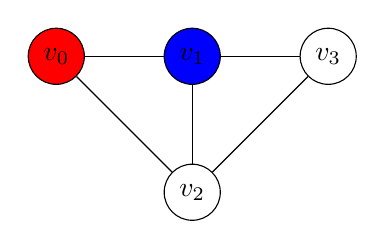
\begin{tikzpicture}[
            every node/.style={circle, draw},
            rouge/.style={red, fill, text=black, draw=black},
            bleu/.style={blue, fill, text=black, draw=black}]
            \node[rouge] (v0)               {$v_0$};
            \node[bleu]  (v1) [right=of v0] {$v_1$};
            \node  (v2) [below=of v1] {$v_2$};
            \node  (v3) [right=of v1] {$v_3$};
            
            \path[-]    (v0) edge (v1)
                        (v0) edge (v2)
                        (v1) edge (v2)
                        (v1) edge (v3)
                        (v2) edge (v3);
        \end{tikzpicture}
    \end{center}
    The reduction encodes the following clauses $C_{2}$, $C_{3,a}$, $C_{3,b}$, $C_{2,3,g1}$ and $C_{2,3,g2}$ corresponding to $v_2$, $v_3$: 
    \begin{itemize}
        \item[-] Let $r_i$, $g_i$, $b_i$ the possible variables for clause $i$
        \item[-] Variables $r_2$, $b_2$, $b_3$ aren't in the clauses because of $X$ (proper colouring conditions)
        \item[-] $C_2 = (g_2) \quad C_{3,a} = (g_3 \vee r_3) \quad C_{3,b} = (\lnot g_3 \vee \lnot r_3) \quad C_{2,3,g1}= (g_2 \vee g_3) \quad C_{2,3,g2}=(\lnot g_2 \vee \lnot g_3)$ 
    \end{itemize}
    The only solution to the 2-SAT problem is:
    \begin{center}
        \{$g_2$: true, $g_3$: false, $r_3$: true, $b_3$: false\}
    \end{center}
    \begin{center}
        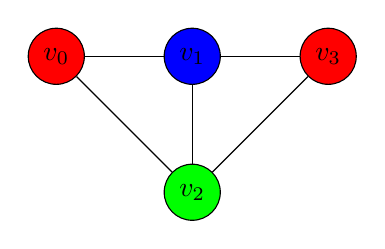
\begin{tikzpicture}[
            every node/.style={circle, draw},
            rouge/.style={red, fill, text=black, draw=black},
            bleu/.style={blue, fill, text=black, draw=black},
            vert/.style={green, fill, text=black, draw=black}]
            \node[rouge] (v0)               {$v_0$};
            \node[bleu]  (v1) [right=of v0] {$v_1$};
            \node[vert]  (v2) [below=of v1] {$v_2$};
            \node[rouge]  (v3) [right=of v1] {$v_3$};
            \path[-]    (v0) edge (v1)
                        (v0) edge (v2)
                        (v1) edge (v2)
                        (v1) edge (v3)
                        (v2) edge (v3);
        \end{tikzpicture}
    \end{center}    
    \underline{Reduction:}\\   
    \emph{We define the following:}
    \begin{itemize}
        \item[-] Let $X$ a coloured dominating set of $G$
        \item[-] Let $r, g, b$ be the 3 different colours
        \item[-] Let $\phi$ the colouring map
        \item[-] $\forallvingnotx$, let $r_v, g_v, b_v \in \mathbb{B}$ the colouring variables
        \item[-] $\forallvingnotx$, let $C_{v,a}$ and $C_{v,b}$ the 2-clauses corresponding to $v$ and the dominating neighbours
        \item[-] $\forall v,w \in V(G)\backslash X$ such that $vw \in E(G)$, let $C_{v,w,c1}$ and $C_{v,w,c2}$ with $c$ a colour, the 2-clauses for non dominating neighbors
    \end{itemize}
    \emph{We have the following properties:}
    \begin{enumerate}[1.]
        \item $\forall v \in X$ $\phi(v) \in \{r, g, b\}$
        \item Let $x \in X$, $\forall v \in N_G(x)$ the proper colouring condition imposes:
        \begin{center}
            $C_{v,\_}$ must not contain $\phi(x)$
        \end{center}
    \end{enumerate}
    To ensure the reduction we need to build $\forall v \in G$ their corresponding clauses in a way that finding a valid solution to the 2-SAT problem:
    \begin{center}
        $\bigwedge\limits_{v \in V(G)\backslash X} (C_{v,1} \wedge C_{v,2} \bigwedge\limits_{w \in N_G(v)\backslash X}(C_{v,w,c1}\wedge C_{v,w,c2}\wedge C_{v,w,d1}\wedge C_{v,w,d2}))$ with $d$, $c$ colours
    \end{center}
    extends properly the colouration of $X$ to $G$. Let $v \in V(G)\backslash X$. At the begining $\forall w \in N_G(v)\backslash X \quad \forall c\in \{r,g,b\}, \quad C_{v,1} = C_{v,w,c1} = (r_v \vee g_v \vee b_v)$ and $C_{v,2} = C_{v,w,c2} = (\lnot r_v \vee \lnot g_v \vee \lnot b_v)$. Then $\forall x \in N_G(v) \cap X$ we apply property $2.$ and we remove $\phi(x)_v$ and $\lnot \phi(x)_v$ from every clause. Since $X$ is a dominating set of $G$, it exists such $x$. If there are two neighbours of $v$ with different colours in $X$ we must remove the negative clause. If there are three neighbours of $v$ with different colours in $X$, the extension is impossible. Then for the remaining $w \in N_G(v)\backslash X$ we remove $C_{v,w,c}$ empty clauses. Since it remains at most 2 available colours, there must be at most 4 clauses. This ensures a correct polynomialreduction.
    \item \emph{Definitions:}
    \begin{itemize}
        \item[-] Let $T$ be the tree created by the BFS algorithm on $G$.
        \item[-] Let $S_1$ and $S_2$ be two vertices sets
        \item[-] Let $<_a$ be the partial order on trees for ancestry  
    \end{itemize}
     $|V(G)| \geq 2$ so there are at least two layers in $T$. We split the tree according to the layer number: first set $S_1$ is composed of even vertices layers and the second set $S_2$ is composed of odd vertices layers. Ensuring the following:
    \begin{center}
        $\forall v, w \in S_i $ s.t $layer(v) < layer(w)$ we have $ v <_a w$
    \end{center}
    Because $T$ is made with the BFS algorithm, every shortest path from a node to its ancestors is in $T$. In other terms, edges $e$ such that $e \in E(G)\backslash E(T)$ cannot link a node with one of its ancestors. So links between layers of the same set are all in $T$. So the two dominating sets are disjoint.\\
    We claim $n/2$ is a tight upper bound. It's an upper bound because we proved that one can split a graph in two dominating sets. It's tight because even filiform graphs have a minimal dominating set size of $n/2$:
    \begin{center}
        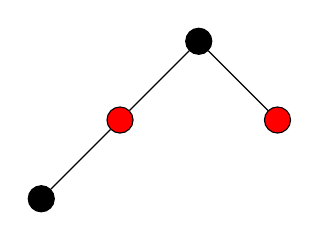
\begin{tikzpicture}[
            every node/.style={circle, draw},
            set1/.style={red, fill, text=black, draw=black},
            set2/.style={black, fill, text=white}]
            \node[set2] (v0) at (2,2) {};
            \node[set1] (v1) at (1,1) {};
            \node[set1] (v2) at (3,1) {};
            \node[set2] (v3) at (0,0) {};
            \path[-]    (v0) edge (v1)
                        (v0) edge (v2)
                        (v1) edge (v3);
        \end{tikzpicture}
    \end{center}    
    \item Let's derive an algorithm that solves 3-COLOUR:
    \begin{algorithm}[H]
        \caption{$O^*((\sqrt{3})^n)$ algorithm to solve 3-COL problem}    
        \begin{algorithmic}
            \State $T \gets BFS(G)$
            \State $S1, S2 \gets bipartiteDominatingSet(T)$
            \If{size($S1$) $<$ size($S2$)}
                \State $X \gets S1$
            \Else
                \State $X \gets S2$
            \EndIf
            \State $\phi \gets colourize(X)$
            \State $\phi \gets reduction2SAT(X, G, \phi)$
        \end{algorithmic}
    \end{algorithm}
    The BFS algorithm is polynomial, defining the two dominating sets is also polynomial (question above). Then we proved that the upper bound for the smallest dominating set is $n/2$ so if we try every colouring possibility on the smallest dominating set we have $3^{\frac{n}{2}} = (\sqrt{3})^n$ possibilities, and the reduction to 2-SAT is also polynomial such as 2-SAT. So the algorithm complexity is indeed $O^*((\sqrt{3})^n)$.
\end{enumerate}
\begin{Question}
    Let us now attack the general k-COLOUR problem.
\end{Question}
\begin{enumerate}[(a)]
    \item $Y = X \cup $
    \item Let's derive an algorithm that solves 3-COLOUR:
    \begin{algorithm}[H]
        \caption{$O(3^n)$ algorithm to solve 3-COL problem}    
        \begin{algorithmic}
            \State colour the graph
        \end{algorithmic}
    \end{algorithm}
\end{enumerate}
\end{document}